\chapter{Steam and the Dataset} \label{sec:BG}

\section{The Steam Platform} \label{sec:BG_Steam}

Steam is a digital distribution platform for video games run by Valve Corporation an American video game publisher. It is the largest of its kind on the PC platform \cite{SteamLargestDistributor} with most of its popular competitors also being run by large video game publishers: Origin by EA and the Epic Games Store by Epic \cite{SteamCompetitors}.

As of January 2022, there are over 60 thousand video games available in the Steam store \cite{SteamGameCount} while the platform boasts over 120 million monthly active users \cite{SteamMonthlyUsers} and over 20 million concurrent users on average \cite{SteamConcurrentUsers}. The service is primarily used as a desktop application which is available on Windows, Mac and Linux although most of the service's functionality can also be found on its website. Games can be purchased, installed and launched all from within the desktop application. Steam also provides publishers with a means to pre-release unfinished games to users as a form of alpha or beta testing. These games are referred to as `Early Access' releases.

The desktop application can be split into four broad categories: the store, the community section, a user's library and a user's profile/management area.

\subsection{Store} \label{sec:BG_Steam_Store}

Games on Steam vary wildly in price with more expensive games being published by triple-A studios and cheaper games being published by smaller, independent developers \cite{SteamGamePricing}. There are over seven thousand free-to-play games available in the store \cite{SteamFreeGameCount}. Users can browse and search for games in the Steam store. Numerous search features are provided to the user including the ability to filter games by their price, their release date, their genres/tags (action, casual, indie, etc) and other characteristics or features of games such as whether or not they support gaming controllers, online multiplayer and so on.

A game's store page contains a large amount of information about itself including both brief and detailed descriptions as well as in-game screenshots and videos. The store page also provides an in-depth list of the aforementioned genres/tags, characteristics and features of the game. An example of the initial section of a game's store page is given in Figure \ref{fig:SteamStore_ApexLegends}.

\begin{figure}[ht]
    \centering
    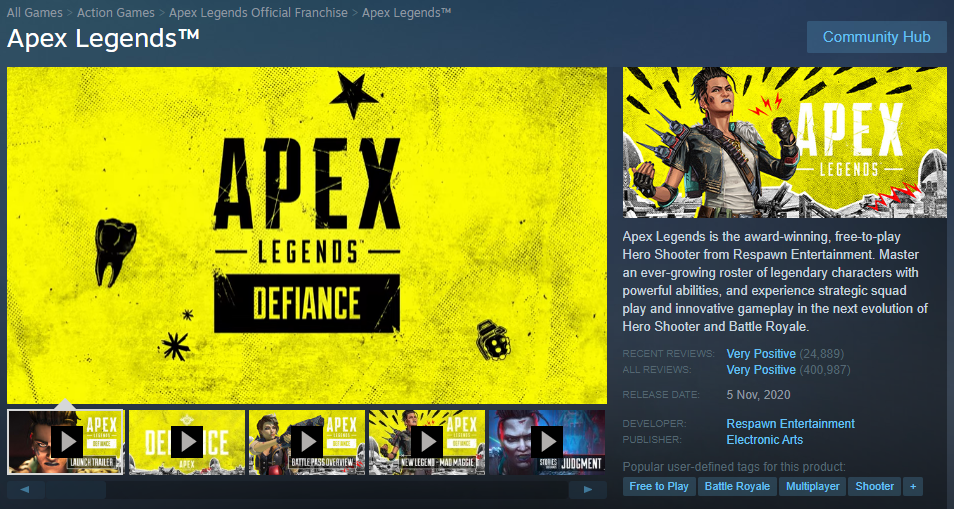
\includegraphics[scale=0.6]{figures/02_background/01_SteamStore_ApexLegends.png}
    \caption{A screenshot of the first section of the Steam store page for the game \textit{Apex Legends}\texttrademark~ \cite{SteamApexLegends}.}
    \label{fig:SteamStore_ApexLegends}
\end{figure}

\subsubsection{Reviews}

Users on Steam can provide reviews for games that they've purchased and played. A game review consists of a simple `thumbs up' or `thumbs down' rating, indicating that the user would or would not recommend the game to other users, as well as some written text. This review system differs from many other platforms which use numerical ratings, eg `out of ten' or `out of five'.

A game's store page will indicate a game's popularity using the percentage of user reviews that were positive (`thumbs up') both in total and over the last 30 days. These percentages are also attached to descriptions such as `Mixed' for a game with, for example, 50\% positive reviews and `Mostly Positive' for a game with 75\% positive reviews. There are also additional popularity descriptors for games with more than a certain number of total reviews. For example, a game with 96\% positive reviews but only 25 reviews in total would be described as `Positive' but a game with the same positive review percentage with 500 total reviews would be described as `Overwhelmingly Positive' \cite{SteamRatingsArticle}. A chart outlining this labelling system, seemingly based on \cite{SteamRatingsArticle}, is given in Figure \ref{fig:SteamStore_Ratings}.

\begin{figure}[ht]
    \centering
    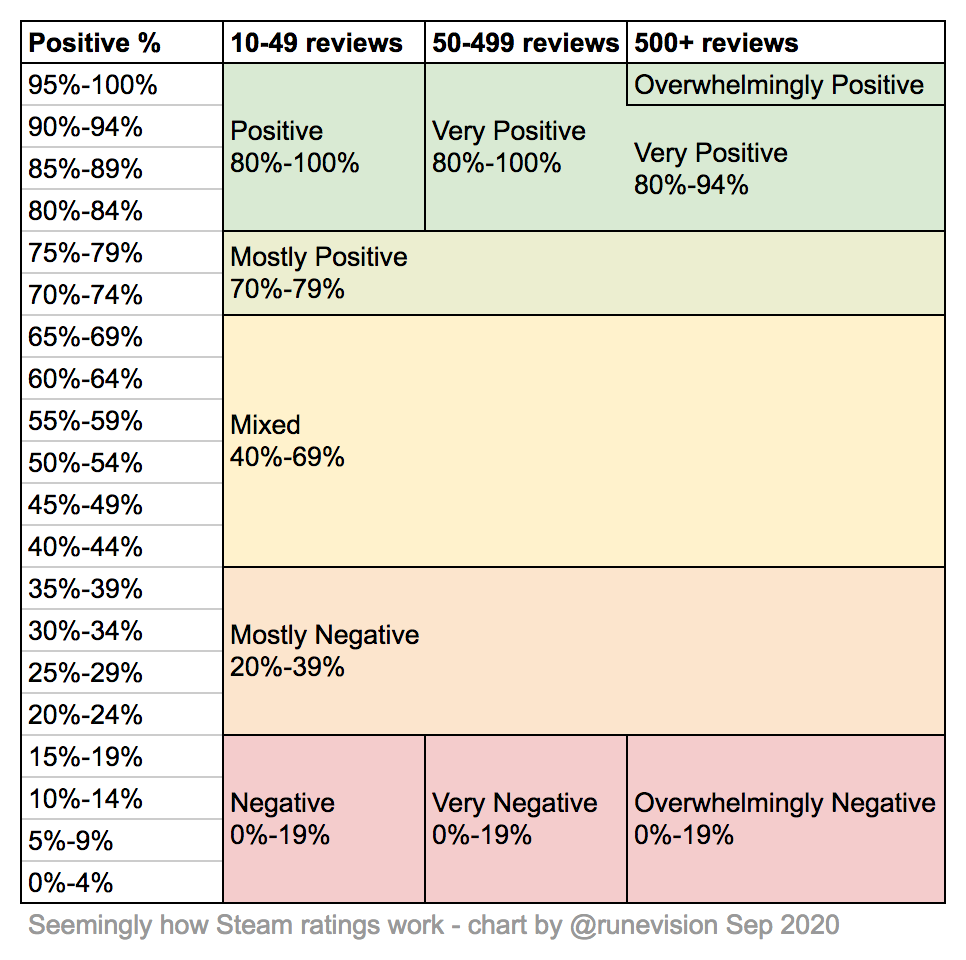
\includegraphics[scale=0.3]{figures/02_background/02_SteamStore_Ratings.png}
    \caption{Steam rating labels by positive review percentage and number of reviews \cite{SteamRatingsChart}.}
    \label{fig:SteamStore_Ratings}
\end{figure}

A certain number of selected reviews and recent reviews are included on a game's store page with an option provided for a user to browse all of that game's reviews on a separate page. Users can give other reviews a `thumbs up' if they found it helpful or a `thumbs down' if they did not, they can also mark a review as `funny' if they found it humorous. The selected reviews that appear on a game's store page are those reviews that received the most `helpful' ratings in the past 30 days.

\begin{figure}[ht]
    \centering
    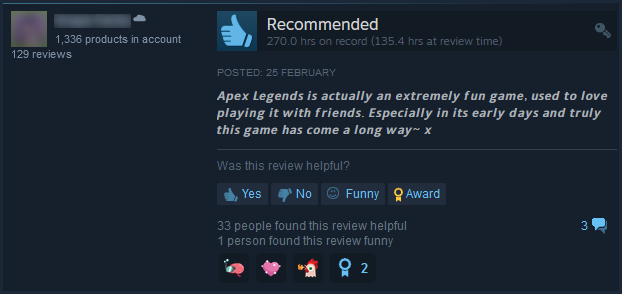
\includegraphics[scale=2.4]{figures/02_background/03_SteamStore_Review.png}
    \caption{A screenshot of a positive review for the game \textit{Apex Legends}\texttrademark~ \cite{SteamApexLegends}.}
    \label{fig:SteamStore_Review}
\end{figure}

As previously mentioned, a review consists of  a `thumbs up' or `thumbs down' rating as well as some written text. However, a review will also list the date that it was written, the amount of time that the user has played the game in total and at the time the review was written. The number of `helpful' and `funny' ratings the review received are also listed. Users can, at a later date, edit both the rating and text of their reviews and information about these edits, if any occurred, is also displayed. When writing a review a user can specify the language the review has been written in although it is not clear if this feature is always used. Finally, a review will also contain a link to the Steam profile of the reviewer as well as information about the number of games that the user owns and the number of reviews they've written. Other users can leave comments on reviews leading to nested discussion threads within the review system.

\subsection{Community} \label{sec:BG_Steam_Comm}

\subsubsection{Community Hubs}

Games on Steam also have what are referred to as `community hubs'. Within these hubs, users can create and participate in discussions on a forum and interact with other users in a chat room. They can also post and share artwork, screenshots and videos related to the game and publish in-game guides and tutorials. The developers of the game can also announce news and updates for their game within this hub. Certain games also support the sharing of game modifications, in-game items and other user-created content within the `Workshop' section of the hub.

\subsubsection{Groups}

Users can also create and join groups on Steam. These groups can be associated with a single game, numerous related games or no game at all. Groups can be discovered in a game's community hub or by using Steam's `find a group' search feature. Group administrators can control the privacy of their group by making them public, private or invite-only. Groups, like community hubs, have discussion forums and chat rooms and group administrators can schedule and host community events.

\subsection{Library} \label{sec:BG_Steam_Lib}

Once a user purchases a game it is added to their library. Users can organise, update or uninstall their games from inside of their library. A game's library page differs from its storefront page. From this page users can view which of their friends are currently playing or have played the game, browse a feed of news, patches and updates related to the game and see a list of in-game achievements and trading cards that they've unlocked. They can also write, edit and view their review of the game. The game's library page also provides direct access to sections of its community hub and there is a search feature present for finding groups related to the game.

\subsubsection{Achievements}

Achievements are rewards specified by a game's developers that are unlocked on Steam (outside of the game itself) usually upon completing particularly difficult sections of or tasking within a game.

\subsubsection{Trading Cards}

Trading cards are virtual items awarded to users in a somewhat random fashion as they play and progress through a particular game. Each game has a certain number of trading cards that users can collect and certain rewards are given to users upon collecting a game's full `set' of trading cards. By design, an individual user will not be able to collect every card on their own and will have to trade or purchase cards from other players of the game on a trading-specific market and forum. The rewards given to users upon completing a set of trading cards will be discussed in the sections that follow.

\subsection{User Profile} \label{sec:BG_Steam_Profile}

Each user has access to their own customisable Steam profile. Depending on the user in question's privacy settings, this profile can be viewed by any other user, their friends or nobody at all. Users can customise many aspects of their profile including their username, profile picture, location and a short description of themselves. A profile can be used to showcase, among other things, which games the user has played or what in-game achievements they have earned. Other users can also leave comments on a user's profile page.

Users can earn `experience points' on Steam in order to increase their profile's `level'. This level is displayed on the user's profile and, as a user increases in level, they get access to additional ways to customise their profile. Experience points are gained by completing sets of trading cards, as discussed in the previous section, by purchasing and playing additional games and by simply maintaining their Steam account for long periods of time.

\subsubsection{Friends}

Users can add other users as friends on Steam. Unlike other social networks such as Twitter, a Steam friendship is bidirectional and a friend request must be accepted by the other party before users are considered friends. The number of friends a user can have is initially limited to 250 but this cap is increased by five each time the user gains another level on Steam.

If two users are friends they can send direct messages to each other, invite each other to games that support multiplayer and view each other's in-game activity.

\section{The Dataset} \label{sec:BG_Dataset}

The dataset used in this project was gathered by Professor Douglas Leith at Trinity College Dublin using a custom-built web scraper written in Python that uses the Scrapy library. The dataset contains comprehensive review, friendship and group membership data for a large number of Steam users. Data is stored using the JSON Lines format where each line or entry in a data file contains a single record, eg a single user's friend data, stored in the form of a JSON object. In its raw form, the dataset contains almost 23 GB of data.

The dataset is split into four parts: reviews, review texts, friends and groups. The review data contains information about all of the reviews left by a particular user excluding the actual text of the review. The review text data contains the corresponding text data for all of the aforementioned users and reviews. The friend data contains a list of all of the friends a particular user has while the group data contains a list of all of the groups the user is a member of.

In total, the dataset contains full review, friendship and group membership data for 4,000,033 individual users. All users in the dataset without at least one review and one friend are excluded in the aforementioned count and in all later work.

\subsection{Steam User IDs} \label{sec:BG_Dataset_UIDs}

Every user on Steam is given a unique user ID in the form of a 17 digit number. The URL that leads to a user's profile relies on this user ID as opposed to, for example, their username. In the case of our dataset, and potentially across Steam as a whole, only the final nine digits of a user's ID appear to vary from user to user while the first eight digits remain constant. These URLs are formatted like so:  \texttt{https://steamcommunity.com/profiles/76561198XXXXXXXXX}. Throughout the dataset, users are identified by the \texttt{profiles/76561198XXXXXXXXX} section of their profile URL.

\subsection{Reviews} \label{sec:BG_Dataset_Revs}

Each entry in this section of the dataset contains an indicator that the entry concerns review data, the Steam user ID for the user in question as well as an array containing data for each of the reviews they've left. Each of the entries in the review array contains the following information:

\begin{itemize}
    \item the unique ID of the game being reviewed;
    \item the polarity of the review (`thumbs up' or `thumbs down');
    \item whether or not the review was for an early access game;
    \item the number of hours the user has played the game in total;
    \item the number of hours the user had played the game when the review was written;
    \item the date (as a string) that the review was written as well as the corresponding Unix timestamp;
    \item if the review was later edited by the user: the date and timestamp that the editing occurred;
    \item the number of `helpful' votes the review received;
    \item the number of `funny' votes the review received; and
    \item the user-specified language that the review was written in.
\end{itemize}

An example entry can be seen in Listing \ref{lst:ExampleData_Review}.

\lstinputlisting[caption={An example of review data for a user with a single written review.},captionpos=b,label={lst:ExampleData_Review}]{listings/02_background/ExampleData_Review.json}

\subsection{Review Texts} \label{sec:BG_Dataset_Texts}

As was the case with the reviews data, each entry in this section contains an indicator that the entry concerns review text data, the Steam user ID of the user in question and an array containing data for each of the user's reviews. Each entry in this array contains the unique ID of the game being reviewed and the review's text content. An example entry can be seen in Listing \ref{lst:ExampleData_ReviewText}.

\lstinputlisting[caption={An example of review text data for a user with a single written review.},captionpos=b,label={lst:ExampleData_ReviewText}]{listings/02_background/ExampleData_ReviewText.json}

\subsection{Friends} \label{sec:BG_Dataset_Friends}

Each entry in this section contains an indicator that the entry concerns friend data, the Steam user ID of the user in question and an array consisting of the user IDs of all of their friends. An example entry can be seen in Listing \ref{lst:ExampleData_Friend}.

\lstinputlisting[caption={An example of friend data for a user with two friends.},captionpos=b,label={lst:ExampleData_Friend}]{listings/02_background/ExampleData_Friend.json}

\subsection{Groups} \label{sec:BG_Dataset_Groups}

Each entry in this section contains an indicator that the entry concerns group data, the Steam user ID of the user in question and an array consisting of the Steam community URLs for each of the groups the user is a member of. An example entry can be seen in Listing \ref{lst:ExampleData_Group}.

\lstinputlisting[caption={An example of group data for a user who is a member of two groups.},captionpos=b,label={lst:ExampleData_Group}]{listings/02_background/ExampleData_Group.json}

\subsection{Conversion to CSV} \label{sec:BG_Dataset_CSV}

To make the data easier to work with in Python they were converted from the JSON Lines format into the CSV format.

\subsubsection{Reviews and Texts}

Steam user IDs were mapped to unique integers counting up from zero and these new IDs were applied to both the friend and group data, too. The review texts and other features were combined into a single row. A sample row of the converted review data is given in Table \ref{tab:ExampleData_Review} while the meanings of the column names are given in Table \ref{tab:ExampleData_Review_Abrv}.

\begin{table}[ht]
    \centering
    \begin{tabular}{l l}
        \toprule
        \textbf{Acronym} & \textbf{Meaning} \\\midrule
        UID & User ID\\
        GID & Game ID\\
        P & Polarity (voted up)\\
        EA & Early access\\
        PT & Playtime in total\\
        PR & Playtime at review\\
        TC & Timestamp at creation\\
        TU & Timestamp at update\\
        VU & Votes up\\
        VF & Votes funny\\
        \bottomrule\\
    \end{tabular}
    \caption{Acronyms for converted review column names.}
    \label{tab:ExampleData_Review_Abrv}
\end{table}

\begin{table}[ht]
    \centering
    \begin{tabular}{l l l l l l l l l l l}
        \toprule
        \textbf{UID} & \textbf{GID} & \textbf{P} & \textbf{EA} & \textbf{PT} & \textbf{PR} & \textbf{TC} & \textbf{TU} & \textbf{VU} & \textbf{VF} & \textbf{Text} \\\midrule
        1 & 12 & 1 & 0 & 3.4 & 2.2 & 1649089205 & 1649089205 & 3 & 0 & "Good game"\\
        \bottomrule\\
    \end{tabular}
    \caption{An example of converted review data.}
    \label{tab:ExampleData_Review}
\end{table}

\subsubsection{Friends}

A sample row from the converted friend data is given in Table \ref{tab:ExampleData_Friend}.

\begin{table}[ht]
    \centering
    \begin{tabular}{l l}
        \toprule
        \textbf{User ID} & \textbf{Friend IDs} \\\midrule
        1 & $2,3,4,5$\\
        \bottomrule\\
    \end{tabular}
    \caption{An example of converted friend data.}
    \label{tab:ExampleData_Friend}
\end{table}

\subsubsection{Groups}

Group names were mapped to unique integers counting up from zero. A sample row of the converted group data is given in Table \ref{tab:ExampleData_Group}.

\begin{table}[ht]
    \centering
    \begin{tabular}{l l}
        \toprule
        \textbf{User ID} & \textbf{Group IDs} \\\midrule
        1 & $2,3,4,5$\\
        \bottomrule\\
    \end{tabular}
    \caption{An example of converted group data.}
    \label{tab:ExampleData_Group}
\end{table}
